
%%% Local Variables:
%%% LaTeX-command: "pdflatex --shell-escape"
%%% End:

\documentclass[11pt]{article}
\usepackage[utf8]{inputenc}
\usepackage[T1]{fontenc}
\usepackage{grffile}
\usepackage{longtable}
\usepackage{wrapfig}
\usepackage{rotating}
\usepackage[normalem]{ulem}
\usepackage{amsmath}
\usepackage{textcomp}
\usepackage{amssymb}
\usepackage{capt-of}
\usepackage{hyperref}
\hypersetup{colorlinks=true, linkcolor=magenta}
\setlength{\parindent}{0in}
\usepackage[margin=0.8in]{geometry}
\usepackage[english]{babel}
\usepackage{mathtools}
\usepackage{palatino}
\usepackage{fancyhdr}
\usepackage{sectsty}
\usepackage{engord}
\usepackage{parskip}
\usepackage{minted}
\usepackage{cite}
\usepackage{graphicx}
\usepackage{subcaption}
\usepackage{setspace}
\usepackage[compact]{titlesec}
\usepackage[center]{caption}
\usepackage{placeins}
\usepackage{color}
\usepackage{amsmath}
\usepackage{bm}
\usepackage{todonotes}
\usepackage{pdfpages}
% \titlespacing*{\subsection}{0pt}{5.5ex}{3.3ex}
% \titlespacing*{\section}{0pt}{5.5ex}{1ex}
\author{Luis Antonio Ortega Andrés\\Antonio Coín Castro}
\date{}
\title{Fingerprint Biometrics Lab - Report\\\medskip
\large APRENDIZAJE PROFUNDO PARA PROCESAMIENTO DE INFORMACIÓN BIOMÉTRICA}
\hypersetup{
 pdfauthor={Luis Antonio Ortega Andrés},
 pdftitle={},
 pdfkeywords={},
 pdfsubject={},
 pdflang={Spanish}}}

\begin{document}

\maketitle

\section*{Exercise 1}
\textbf{a) } \emph{Copy here the two fingerprint images provided as examples (\texttt{example1\_1} and \texttt{example1\_2})}.

\begin{figure}[h!]
  \centering
       \begin{subfigure}[t]{0.45\textwidth}
         \centering
         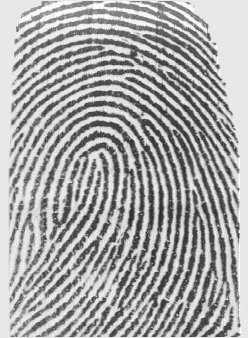
\includegraphics[scale=0.8]{img/example1_1.png}
         \caption{Example1\_1}
     \end{subfigure}%
     \quad
     \begin{subfigure}[t]{0.45\textwidth}
         \centering
         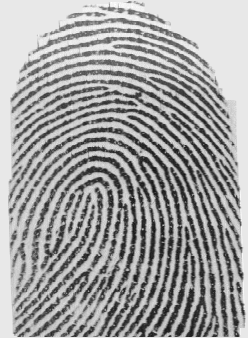
\includegraphics[scale=0.8]{img/example1_2.png}
         \caption{Example1\_2}
     \end{subfigure}
    \caption{Original fingerprints.}
    \label{fig:ex1a}
\end{figure}

\textbf{b) } \emph{How many macro-singularities do you observe in each fingerprint?}

We can see in Figure \ref{fig:ex1a} that there is only one macro-singularity in each fingerprint. Specifically, we observe a \textbf{loop} in each one of them, around the centre of each image. There are no \textit{deltas} or \textit{whorls}.

\textbf{c) } \emph{Mark the macro-singularities in the images (deltas and loops).}

The result of marking each of the loops in shown in Figure \ref{fig:ex1c}. To avoid cluttering the images, we only point out the zones in which the ``U'' shape is most notable.

\begin{figure}[h!]
  \centering
       \begin{subfigure}[t]{0.45\textwidth}
         \centering
         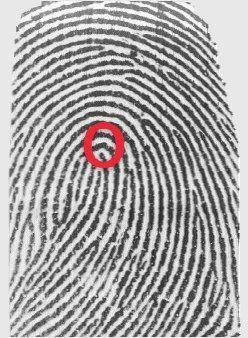
\includegraphics[scale=0.6]{img/msing_1.jpg}
         \caption{Example1\_1}
     \end{subfigure}%
     \quad
     \begin{subfigure}[t]{0.45\textwidth}
         \centering
         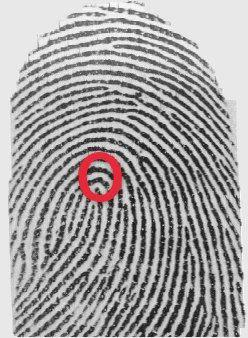
\includegraphics[scale=0.6]{img/msing_2.jpg}
         \caption{Example1\_2}
     \end{subfigure}
    \caption{Macro-singularities (loops).}
    \label{fig:ex1c}
\end{figure}

\newpage
\section*{Exercise 2}

\textbf{a) }\emph{Execute the provided code for Fingerprint Enhancement and paste the resulting image here.}

The resulting image is shown in Figure \ref{fig:ex2a}.

\begin{figure}[h!]
  \centering
       \begin{subfigure}[t]{0.45\textwidth}
         \centering
         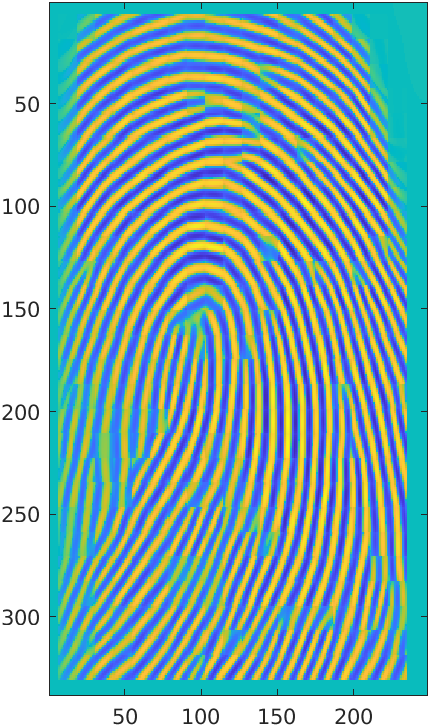
\includegraphics[scale=0.7]{img/enhanced_1}
         \caption{Example1\_1}
     \end{subfigure}%
     \quad
     \begin{subfigure}[t]{0.45\textwidth}
         \centering
         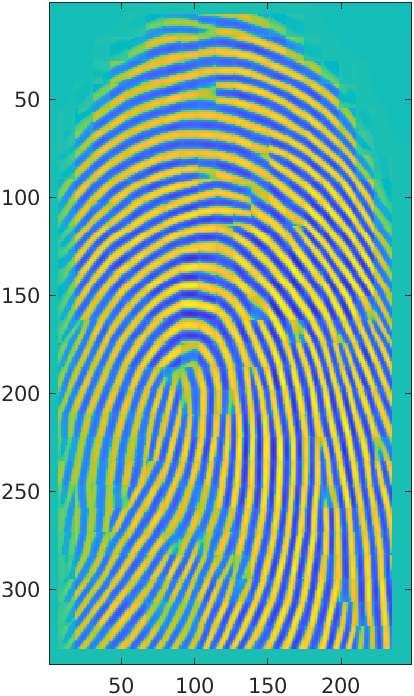
\includegraphics[scale=0.725]{img/enhanced_2}
         \caption{Example1\_2}
     \end{subfigure}
    \caption{Fingerprint Enhancement.}
    \label{fig:ex2a}
\end{figure}


\textbf{b) }\emph{What differences do you observe with respect to the original fingerprints?}

Fingerprint enhancement facilitates the identification of ridge-valley structures and hence the features of each fingerprint. More precisely, we obtain a representation where any intermittent stroke of a ridge is replaced with a continuous one, and also contrast enhancement is performed. As we can see in Figure \ref{fig:ex2a}, the differences with respect to Figure \ref{fig:ex1a} are that the ridge lines are continuous, smoother, and can be distinguished more clearly from the background.\\

\section*{Exercise 3}

\textbf{a) }\emph{Execute now the code for Quality Maps, and paste the resulting quality maps.}

The resulting quality maps are shown in Figure \ref{fig:ex3a}.

\begin{figure}[h!]
  \centering
       \begin{subfigure}[t]{0.45\textwidth}
         \centering
         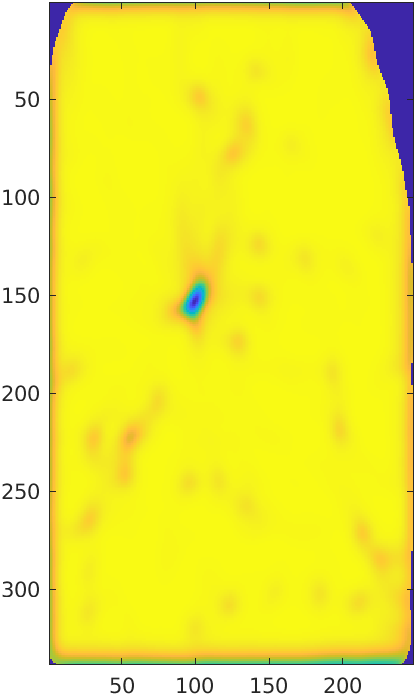
\includegraphics[scale=0.7]{img/qmap_1}
         \caption{Example1\_1}
     \end{subfigure}%
     \quad
     \begin{subfigure}[t]{0.45\textwidth}
         \centering
         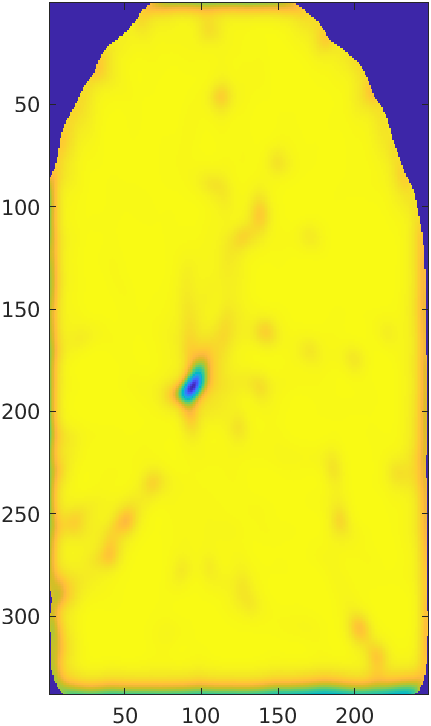
\includegraphics[scale=0.675]{img/qmap_2}
         \caption{Example1\_2}
     \end{subfigure}
    \caption{Fingerprint Quality Maps.}
    \label{fig:ex3a}
\end{figure}

\textbf{b) }\emph{What is the range of values for these quality maps?}

Inspecting each matrix by hand, we can see that for both images the minimum value (shown in dark blue) is \( 0.0 \), while the maximum values (shown in yellow) are \( 0.9991 \) and \(  0.9988 \) for \verb@Example1_1@ and \verb@Example1_2@, respectively. Given this, we can assume that the range of values for the quality is \( [0, 1] \).

\textbf{c) }\emph{What kind information (apart from the quality) can be inferred from such code?}

Inspecting the given source code, we conclude that the heat map displayed in Figure \ref{fig:ex3a}} corresponds to a measure of the reliability of the computed orientation for each ridge (by means of the function \verb@ridgeorient@). We can think of this quantity as a measure of how well the computed orientation resembles the real outline of the ridge curves.

Taking a look at our examples, there is one region in both fingerprints where the reliability is low (blue), which corresponds to the sharpest point of the loop. This phenomenon is to be expected, given that those points are precisely the ones where the orientation changes abruptly, leading to less accurate results.

\newpage

\section*{Exercise 4}

\emph{Execute the code in order to show the Binarized Fingerprint and the Segmented Fingerprint. Apply different values of quality threshold (0.1, 0.3, 0.6, 0.9) and paste here the resulting images.}

The resulting images are shown in Figure \ref{fig:ex4}. First, we plot the binarized fingerprint, that is, a representation where only black-and-white is used (to distinguish the ridge lines from the valleys). Then, we superimpose a mask that delimits the zone of what we can consider a fingerprint (versus the background). Finally, we plot the reliability mask only for the points that exceed a certain reliability threshold.

\begin{figure}[h!]
  \centering
  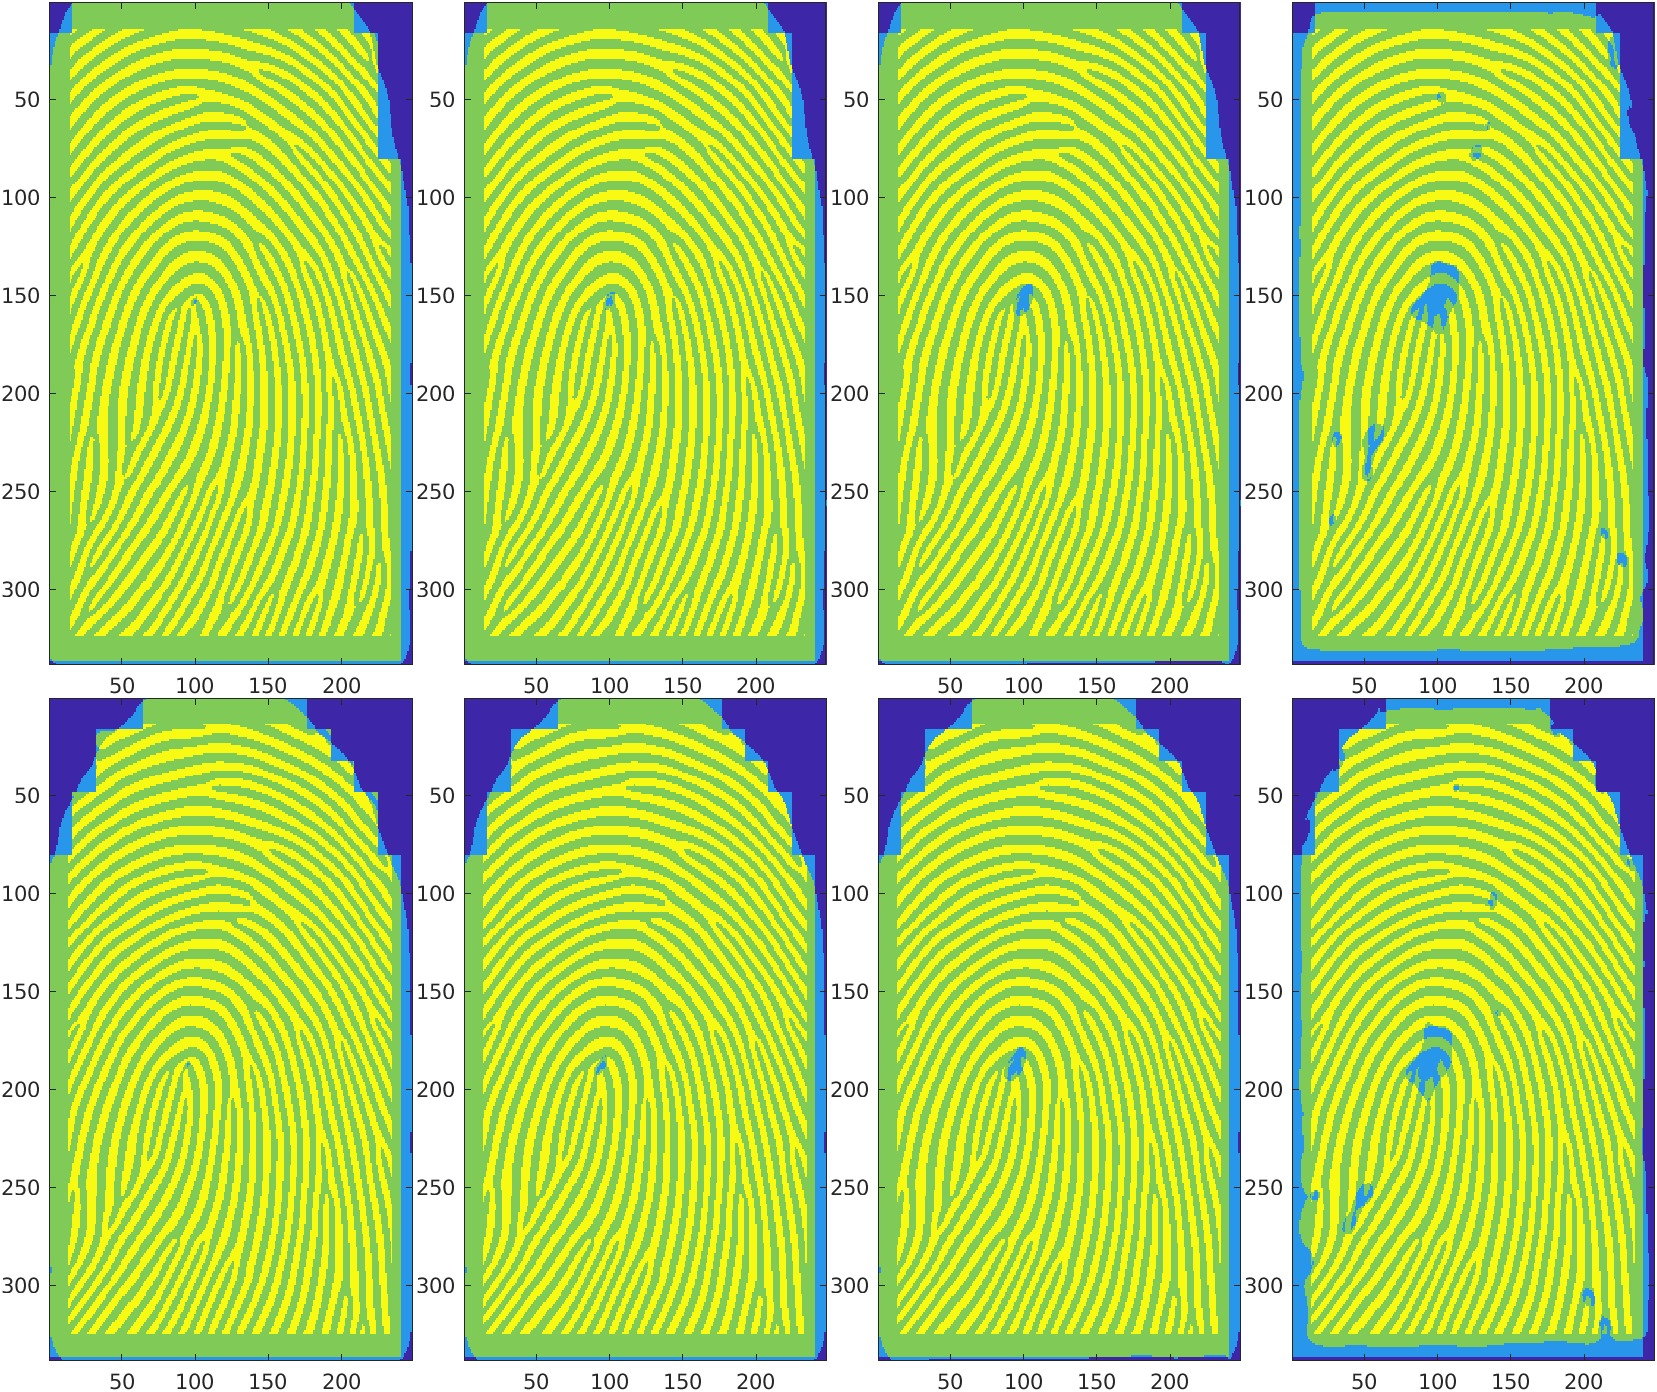
\includegraphics[scale=0.4]{img/merge_bin}
  \caption{Binarized and Segmented fingerprints with thresholds $0.1, 0.3, 0.6$ and $0.9$. The first row corresponds to \texttt{Example1\_1} and the second one to \texttt{Example1\_2}, while the threshold increases from left to right.}
  \label{fig:ex4}
\end{figure}

We can see that as we increase the threshold, more and more points are missing from the final mask (especially the ones around the loops, where the reliability is lower). In the final part of the code, we also ``turn off'' the points that don't pass the threshold test.

\section*{Exercise 5}

\textbf{a) }\emph{Execute the code for generating the Fingerprint Skeleton and the Minutiae Extractor. Paste the resulting images for the original values window=5 and margin=5.}

The Fingerprint Skeleton code aims to make the ridge lines thinner (1px), so that its analysis for extractiig minutiae becomes easier. The Minutiae Extractor then tries to find all relevant minutiae, using a window of a specified size and ignoring the points within a certain distance of the margin of the image. The results are shown in Figure \ref{fig:ex5a}.

We notice that using the default parameters there are several mintuae that are not correctly extracted (in particular, some bifurcations in the first fingerprint are not detected). In addition, we can see that there are many marks in the border of each image, which can be suboptimal, since these minutiae are somewhat artificial and caused by the fact that we don't have a complete image (only a section of the frontal projection of the fingerprint).

\begin{figure}[h!]
  \centering
       \begin{subfigure}[t]{0.45\textwidth}
         \centering
         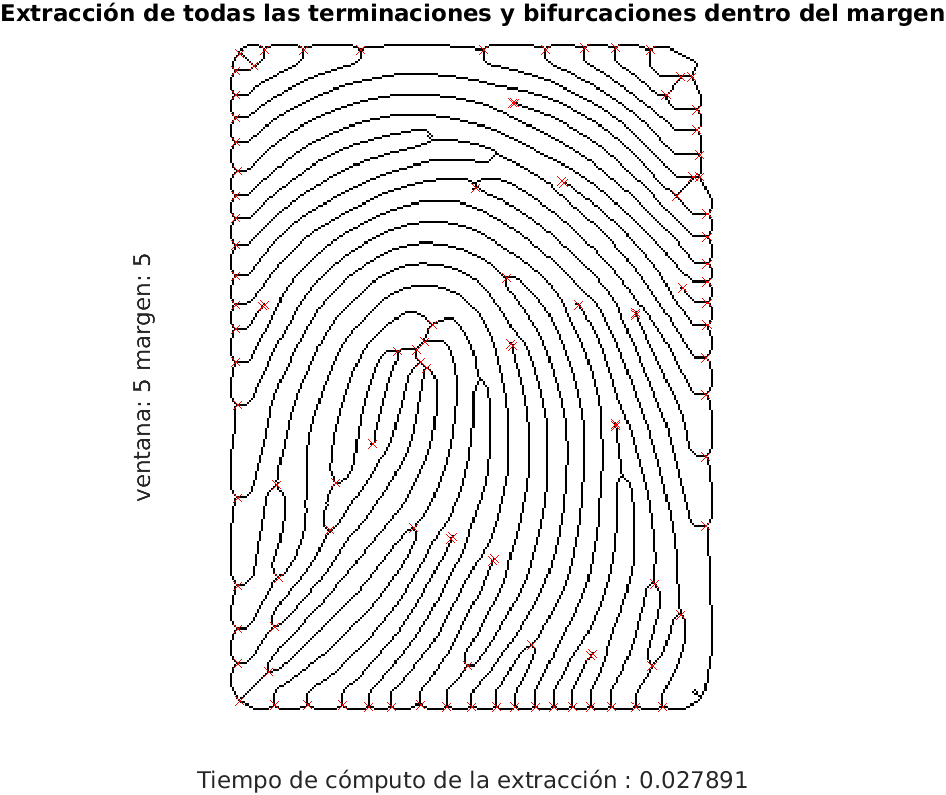
\includegraphics[scale=0.5]{img/extraction_1}
         \caption{Example1\_1}
     \end{subfigure}%
     \quad
     \begin{subfigure}[t]{0.45\textwidth}
         \centering
         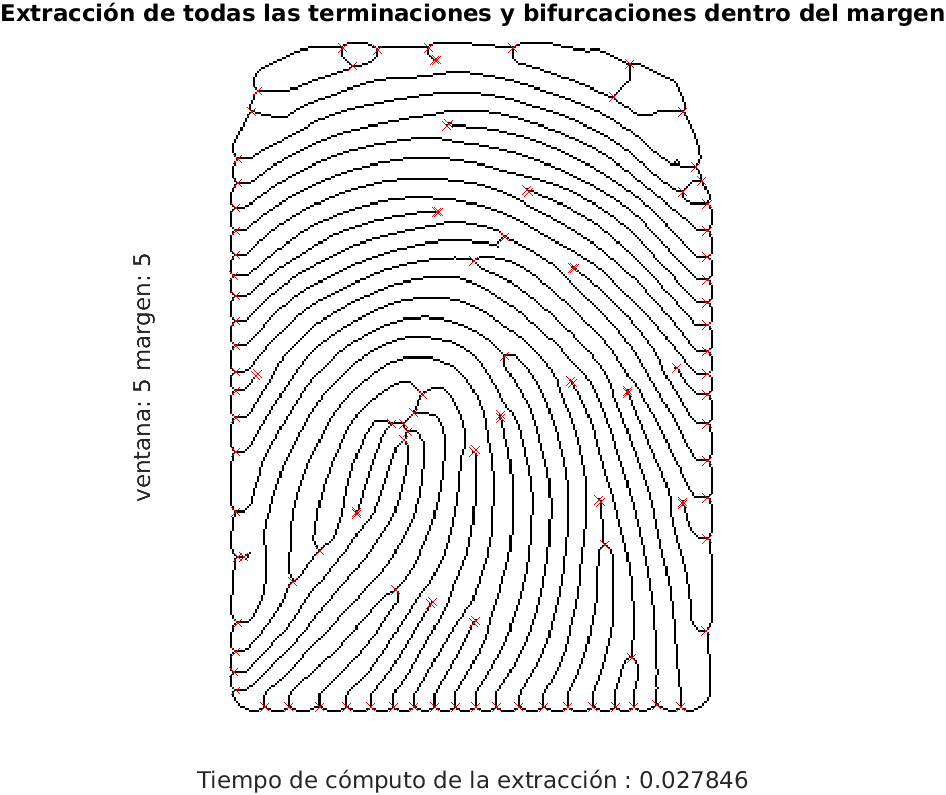
\includegraphics[scale=0.5]{img/extraction_2}
         \caption{Example1\_2}
     \end{subfigure}
    \caption{Fingerprint Skeleton and Minutiae Extractor output with default parameters.}
    \label{fig:ex5a}
\end{figure}

\textbf{b) }\emph{Search heuristically by looking at the images for the optimal values of parameters window and margin. Paste the resulting images with your optimal parameters and justify your decision.}

To solve the problems mentioned above, we search heuristically for the best combination of window and margin values. On the one hand, we found that decreasing the window to $3\times 3$ provided better results (all visible minutiae were detected).

On the other hand, increasing the margin to a higher value alleviated the problem of wrongly detecting minutiae on the border, since the feasible region is moved away from the border. However, we have to be careful not to increase the margin too much, because then we could lose some genuine minutiae that are close to the border. We found that setting the margin to $11$px was a good compromise.

The resulting images are shown in Figure \ref{fig:ex5b}.

\begin{figure}[h!]
  \centering
       \begin{subfigure}[t]{0.45\textwidth}
         \centering
         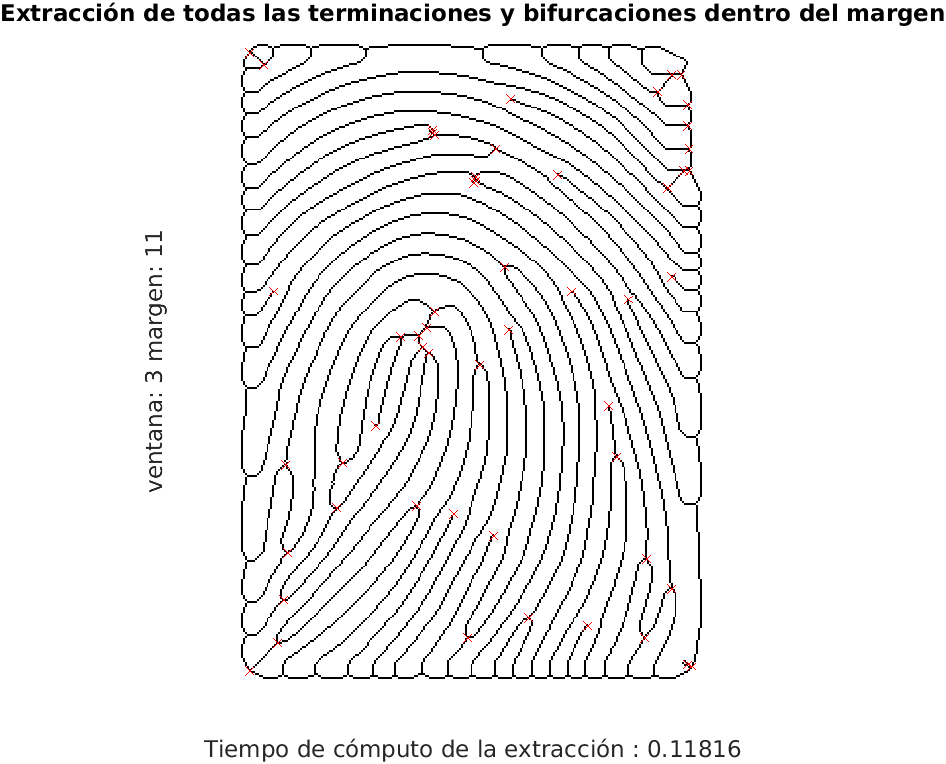
\includegraphics[scale=0.5]{img/extraction_optim_1}
         \caption{Example1\_1}
     \end{subfigure}%
     \quad
     \begin{subfigure}[t]{0.45\textwidth}
         \centering
         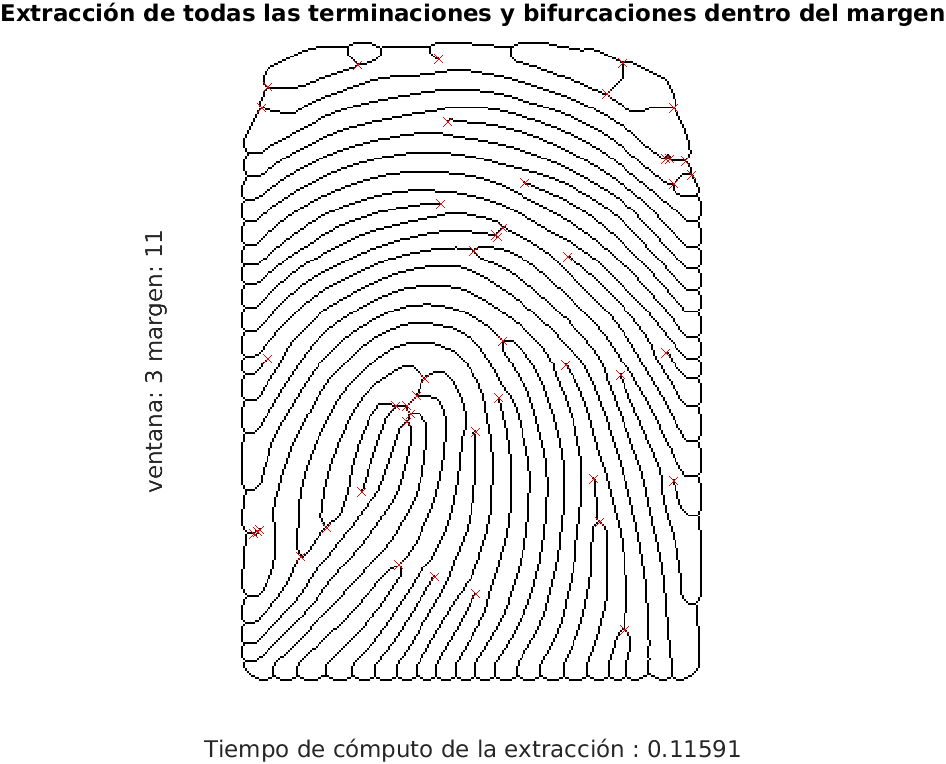
\includegraphics[scale=0.5]{img/extraction_optim_2}
         \caption{Example1\_2}
     \end{subfigure}
    \caption{Fingerprint Skeleton and Minutiae Extractor output with optimal parameters.}
    \label{fig:ex5b}
\end{figure}

\section*{Exercise 6}

\textbf{a) }\emph{Execute the code corresponding to the Minutiae Validation for window=5 and margin=5.  Paste the resulting image including the minutiae extracted (red crosses) and validated (blue circles) of both fingerprints.}

The minutiae extracted and validated with the default extraction parameters are shown in Figure \ref{fig:ex6a}.

\begin{figure}[h!]
  \centering
       \begin{subfigure}[t]{0.45\textwidth}
         \centering
         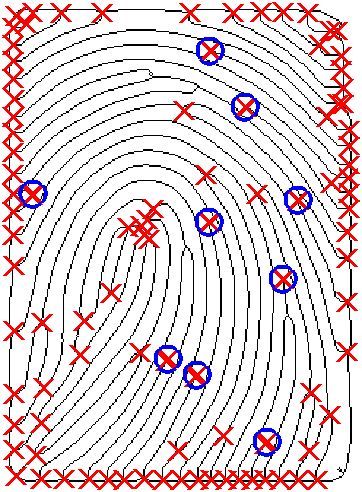
\includegraphics[scale=0.75]{img/ext_val_1}
         \caption{Example1\_1}
     \end{subfigure}%
     \quad
     \begin{subfigure}[t]{0.45\textwidth}
         \centering
         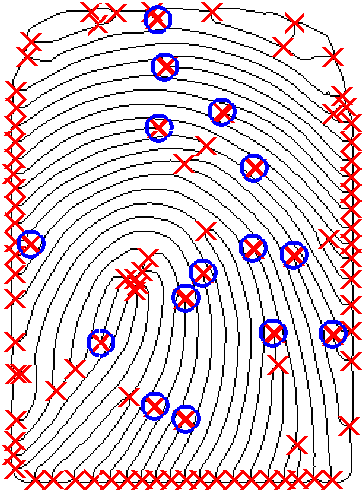
\includegraphics[scale=0.75]{img/ext_val_2}
         \caption{Example1\_2}
     \end{subfigure}
    \caption{Minutiae Validation output with default parameters.}
    \label{fig:ex6a}
\end{figure}

\textbf{b) }\emph{Execute the same code but with the optimal values of parameters window and margin. Paste the resulting image below.}

The minutiae extracted and validated with the optimal extraction parameters are shown in Figure \ref{fig:ex6b}.

\begin{figure}[h!]
  \centering
       \begin{subfigure}[t]{0.45\textwidth}
         \centering
         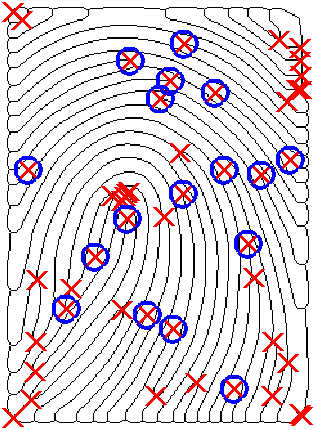
\includegraphics[scale=0.85]{img/ext_val_optim_1}
         \caption{Example1\_1}
     \end{subfigure}%
     \quad
     \begin{subfigure}[t]{0.45\textwidth}
         \centering
         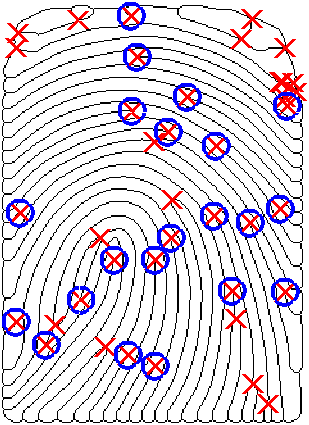
\includegraphics[scale=0.85]{img/ext_val_optim_2}
         \caption{Example1\_2}
     \end{subfigure}
    \caption{Minutiae Validation output with optimal parameters.}
    \label{fig:ex6b}
\end{figure}

\textbf{c) }\emph{Do you think it is a good idea to include the Minutiae Validation module? Justify your opinion.}

It is a good idea, because it allows us to retain only those minutiae that are actually relevant for comparing two fingerprints. It isolates the minutiae so that they are easier to compare (reducing noise), and it also lets us correct the possible (non-)minutiae detected on the border.

\newpage
\section*{Extra Exercise}

\emph{In folder \texttt{/ddbb} you have 20 fingerprint images. 19 of them are labeled with the subject identity (e.g., H0001), and 1 is Unknown. Search for the identity of the Unknown fingerprint in the set of 19 labelled reference fingerprints. You can use the provided code \texttt{identification\_1\_19.m} as basis. Paste here the resulting ranked list of scores of the Unknown fingerprint with respect each one of the 19 reference fingerprints.}

In order to compare each fingerprint in the database with the unknown print, we will extract (and validate) the minutiae of each fingerprint and apply the Hough transform to compute the scores between each one of them and the unknown one. To this end, we use the code already implemented in \verb|Hough.m| and we write a function called \verb|extract_minutiae|:

\begin{minted}{matlab}
function [valid_x,valid_y]=extract_minutiae(I, ew, em, vw)
  ext_window=ew;
  ext_margin=em;
  val_window=vw;
  [~,~,~,~,~,enhI] = fft_enhance_cubs(I, -1);
  [~, binI,~,~, I1_enhaced] = testfin(enhI);
  inv_binI = (binI == 0);
  thin = bwmorph(inv_binI, 'thin', Inf);
  [minutiae, minutiae_x, minutiae_y,~]=extraction(thin,ext_window,ext_margin);
  [valid, valid_x, valid_y,~]=validation(thin,minutiae,val_window);
end
\end{minted}

We have tried a total of 4 combinations of the parameters \verb|window| and \verb|margin| for extraction, and \verb|window| for validation. We decided to modify this last parameter to see how it would influence the result.

\textbf{First attempt.} The first combination of parameters chosen was the same as in Exercise 6 (the optimal extraction parameters and the default validation window):
\[
\{\texttt{extract\_window}=3, \texttt{ extract\_margin}=11, \texttt{ validation\_window}=1\}
\]
We obtained the following scores for each of the 19 fingerprints on the database, shown in Table \ref{tab:1}.

\begin{table}[h!]
  \centering
  \begin{tabular}{ccccccccccc}
    & \textbf{#1} & \textbf{#2} & \textbf{#3} & \textbf{#4} & \textbf{#5} & \textbf{#6} & \textbf{#7} & \textbf{#8} & \textbf{#9} & \textbf{#10}\\
    \hline
    \textbf{Score}& 0.1860 &0.1525 & 0.2045 & 0.1538& 0.1220& 0.1361& 0.1739 &0.2318& 0.1758& 0.1764\\

    & \textbf{#11} & \textbf{#12} & \textbf{#13} & \textbf{#14} & \textbf{#15} & \textbf{#16} & \textbf{#17} & \textbf{#18} & \textbf{#19}\\
    \hline
    \textbf{Score} & 0.1333& 0.2000& \textbf{{\color{red}0.5500}} &0.1978 &0.1587& 0.1975 &0.2040& 0.1269 &0.2022
\end{tabular}
\caption{Hough scores for each fingerprint in the first attempt.}
\label{tab:1}
\end{table}

As we can see, the fingerprint number 13 is the winner, obtaining a coincidence score of $55\%$, way ahead of the rest of the prints.

\textbf{Second attempt.} Next, we decided to slightly increase the validation window:
\[
\{\texttt{extract\_window}=3, \texttt{ extract\_margin}=11, \texttt{ validation\_window}=3\}
\]
The scores obtained are displayed on Table \ref{tab:2}. In this case, the score of fingerprint $\#13$ increases to $65\%$, while the scores for the rest of the prints remain relatively low.

\begin{table}[h!]
  \centering
  \begin{tabular}{ccccccccccc}
    & \textbf{#1} & \textbf{#2} & \textbf{#3} & \textbf{#4} & \textbf{#5} & \textbf{#6} & \textbf{#7} & \textbf{#8} & \textbf{#9} & \textbf{#10}\\
    \hline
    \textbf{Score}& 0.2598& 0.2295& 0.2645& 0.2153& 0.1964& 0.1951& 0.2237& 0.2614& 0.2241& 0.2033\\

    & \textbf{#11} & \textbf{#12} & \textbf{#13} & \textbf{#14} & \textbf{#15} & \textbf{#16} & \textbf{#17} & \textbf{#18} & \textbf{#19}\\
    \hline
    \textbf{Score} & 0.2044& 0.2352& \textbf{\color{red}0.6542}& 0.2362& 0.2039& 0.2289& 0.2311& 0.2000& 0.2393
\end{tabular}
\caption{Hough scores for each fingerprint in the second attempt.}
\label{tab:2}
\end{table}

\newpage
\textbf{Third attempt.} Finally, we thought we would try to decrease the value of the extraction margin, since we had increased it quite a bit from the default value:
\[
\{\texttt{extract\_window}=3, \texttt{ extract\_margin}=7, \texttt{ validation\_window}=3\}
\]

The scores obtained are shown in Table \ref{tab:3}. As we can see, with this combination of parameters we obtain an even higher score for fingerprint $\#13$, which reaches $76\%$ of coincidence. The downside with this approach is that the scores for the rest of the fingerprints are also higher, but they still remain low enough in comparison to the winner.

\begin{table}[h!]
  \centering
  \begin{tabular}{ccccccccccc}
    & \textbf{#1} & \textbf{#2} & \textbf{#3} & \textbf{#4} & \textbf{#5} & \textbf{#6} & \textbf{#7} & \textbf{#8} & \textbf{#9} & \textbf{#10}\\
    \hline
    \textbf{Score}& 0.3237& 0.2616& 0.2857& 0.2816& 0.2636& 0.2800& 0.2872& 0.2978& 0.3061& 0.2515\\

    & \textbf{#11} & \textbf{#12} & \textbf{#13} & \textbf{#14} & \textbf{#15} & \textbf{#16} & \textbf{#17} & \textbf{#18} & \textbf{#19}\\
    \hline
    \textbf{Score} & 0.2735& 0.2857& \textbf{{\color{red}0.7666}}& 0.3377& 0.2827& 0.2685& 0.2876& 0.2649& 0.2789
\end{tabular}
\caption{Hough scores for each fingerprint in the third attempt.}
\label{tab:3}
\end{table}

For this third attempt, we show in Figure \ref{fig:final-minutiae} the validated minutiae for the unkown fingerprint and image number 13, where we can see the coincidences. Based on the previous discussion, we are quite sure that \textbf{the unkown fingerprint corresponds to the 13th fingerprint on the database}.
\begin{figure}[h!]
  \centering
       \begin{subfigure}[t]{0.45\textwidth}
         \centering
         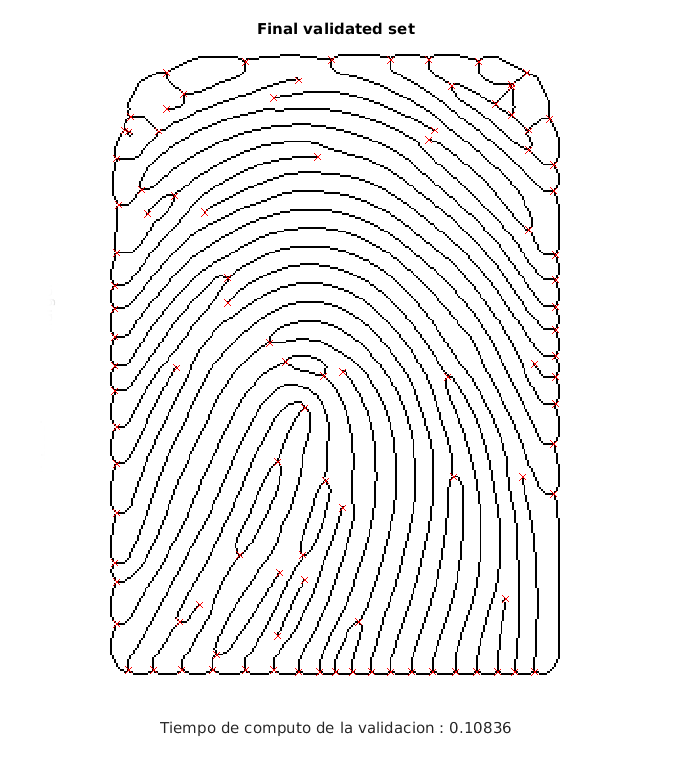
\includegraphics[scale=0.425]{img/unknown_3-7-3}
         \caption{Unknown fingerprint}
     \end{subfigure}%
     \quad
     \begin{subfigure}[t]{0.45\textwidth}
         \centering
         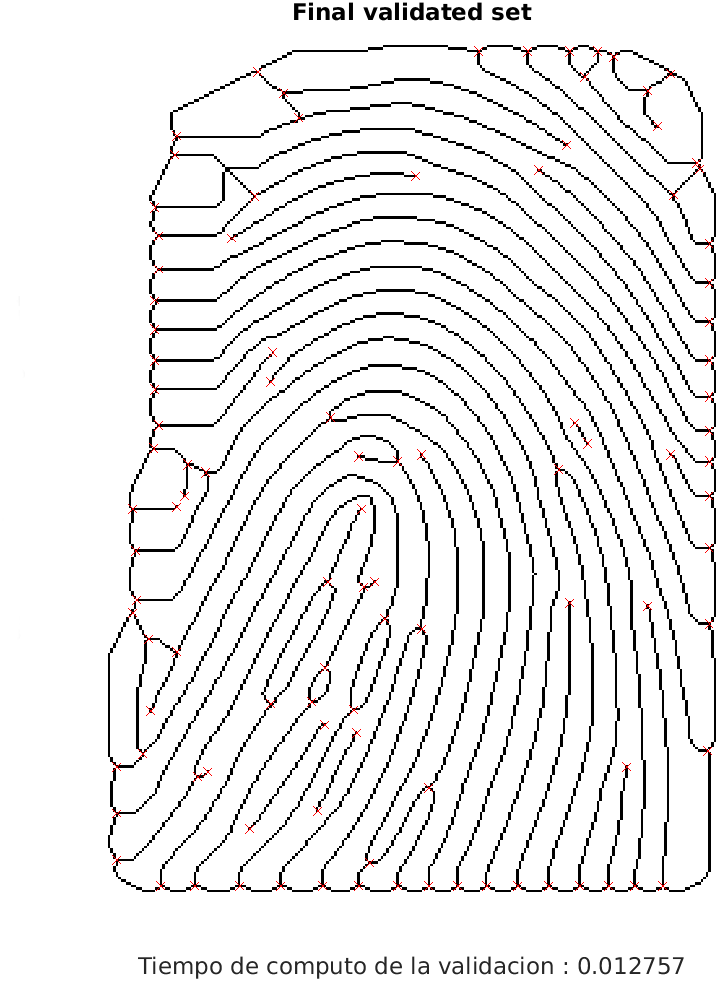
\includegraphics[scale=0.5]{img/13_3-7-3}
         \caption{Fingerprint 13}
     \end{subfigure}
    \caption{Extracted and validated minutiae in the third attempt.}
    \label{fig:final-minutiae}
\end{figure}

\end{document}
